\section{Experiments}\label{sec:exp}

\subsection{Setup}\label{sec:exp_setup}

\paragraph{Models and budgets.}
We evaluate LLaMA-2-7B-Chat, LLaMA-2-13B-Chat, and
Vicuna-13B-v1.5~\cite{touvron2023llama2,chiang2023vicuna}, three
instruction-tuned decoders whose native context window is 4K tokens;
LLaMA-2-Chat is aligned with human-feedback training in the lineage of
instruction-following models~\cite{ouyang2022training} and Vicuna-13B-v1.5
fine-tunes the same LLaMA-2 base with a supervised conversational
recipe, so the three models span alignment lineages rather than base
pretraining runs. Perplexity is reported for all three models; the
LongBench, retrieval, and generation evaluations use the 13B model,
which is the configuration the community deploys for these benchmarks.
The main comparison uses a $20\%$ budget, and the budget sweep covers
$10\%$, $20\%$, and $50\%$. SAGE uses one configuration everywhere:
$\rho = 0.2$, $r = 32$, $\lambda = 0.99$, $K = 512$, $\tau = 1.5$,
$|\mathcal{S}| = 4$; the only input is the contract $\rho$.

\paragraph{Baselines.}
We compare against the full cache, StreamingLLM with 4 sinks and a
window of the budgeted size~\cite{xiao2023efficient}, H2O run in its
official hybrid split, a heavy-hitter ratio of 0.1 plus a recent-token
ratio of 0.1 under the same total budget~\cite{zhang2023h2o},
ScissorHands~\cite{liu2023scissorhands}, TOVA capped at the contract
(a stated departure from its native budget-free protocol, which we
discuss with the results), and FastGen with pattern-specific
strategies~\cite{ge2023model}. Every baseline received the same tuning
budget as SAGE, and the tuned configurations follow their papers;
Table~\ref{tab:hyper} lists the final values.
KIVI~\cite{liu2024kivi} compresses bytes rather than entries, so we
discuss it separately from the entry-count comparison.

\paragraph{Benchmarks and metrics.}
Language quality is the perplexity of WikiText-2~\cite{merity2016pointer}
and PG19~\cite{rae2019compressive} under a sliding window of 2048
tokens, averaged over three seeds with standard deviations; both are
held-out language-modeling benchmarks whose domains are disjoint from
web-scale pretraining collections such as the
Pile~\cite{gao2020pile}. Long-context
ability is the eleven-task LongBench suite~\cite{bai2023longbench} in
its English configuration. Retrieval is measured by a
needle-in-a-haystack protocol~\cite{liu2023lost} that buries one fact at
four depth positions of contexts from 8K to 128K tokens and reports the
accuracy of returning it, 50 samples per cell. Efficiency reports peak
KV memory, prefill latency, and decode throughput on one A100-40GB
with batch size 1, plus the maximum context that fits a 24 GB GPU.
Generation quality under compression is sampled with
MT-Bench~\cite{zheng2023judging} in the appendix. The complete compute
account is 8 A100-40GB GPUs for about 420 GPU-hours including baseline
tuning; hyperparameter search ranges appear in
Table~\ref{tab:hyper}.

\paragraph{Protocol for contexts beyond the native window.}
All methods, including the full-cache reference, run under the same
position extension: NTK-aware interpolation of the rotary
embeddings~\cite{peng2023yarn} with scaling factor $\alpha = 8$ applied uniformly before any cache
policy takes effect, so the extension is a constant of the comparison
rather than a per-method choice. LongBench inputs are truncated to the
model's effective window from the left, preserving the document tail
where most questions anchor. Needle haystacks are built from Paul
Graham essays as filler, with three distractor facts inserted at
different depths and the target needle placed at one of four depth
positions; the question is always the final segment, and the model must
return the exact bound value. The same prompt template, decoding
temperature of $0.0$, and greedy sampling are used for every method.

\paragraph{Statistical methodology.}
Every perplexity and LongBench number is the mean over three seeds
$\{42, 123, 2024\}$ that fix sampling, data order, and the RNG state of
the eviction policy; shaded bands in all line figures are one standard
deviation across seeds, and table entries carry the standard deviation
in the released record. We report the standard deviation rather than
the standard error because the seeds vary the policy trajectory, not an
estimate of a population mean, and the spread across policy trajectories
is the quantity a deployment should plan against. Needle cells average
50 samples per depth-position combination.
Efficiency numbers are single-run measurements on an isolated GPU, and
repeated runs vary by less than $1\%$, so we do not report error bars
for them. Because the needle cells average four depths of 50 samples,
the depth-averaged binomial standard error is at most $1.6$ points at
$n = 200$, while the single-cell error at $n = 50$ reaches $3.1$ points
at $94.8\%$ accuracy and $5.5$ points at $81.6\%$. We therefore read
the SAGE-versus-baseline retrieval gaps, $13.2$ points over TOVA and
$16.6$ over H2O at 128K, as clear of the noise floor, while the
full-cache-versus-SAGE gap of $3.3$ points at 128K is only about twice
the depth-averaged spread and we do not claim it as a significant
difference. No other comparison in the paper rests on a gap smaller
than twice the corresponding spread.

\subsection{Language quality under compression}\label{sec:exp_ppl}

This experiment tests claim C1, that SAGE holds language quality near
the full cache at aggressive budgets. Table~\ref{tab:main} reports the
perplexity of all methods at a $20\%$ budget on the three models, and
Table~\ref{tab:sweep} together with Figure~\ref{fig:ppl} sweeps the
budget on LLaMA-2-7B-Chat.

\begin{table}[t]
\centering
\caption{Perplexity of all methods at a $20\%$ KV budget on three
models (mean over 3 seeds; std is at most $0.31$ and is reported in
the released record). The Full row is the uncompressed reference.
Lower is better. The best compressed value per column is set in
boldface.}
\label{tab:main}
\small
\begin{tabular*}{\textwidth}{@{\extracolsep{\fill}} l cccccc}
\toprule
& \multicolumn{2}{c}{LLaMA-2-7B} & \multicolumn{2}{c}{LLaMA-2-13B}
& \multicolumn{2}{c}{Vicuna-13B} \\
\cmidrule(lr){2-3}\cmidrule(lr){4-5}\cmidrule(lr){6-7}
Method & Wiki-2 & PG19 & Wiki-2 & PG19 & Wiki-2 & PG19 \\
\midrule
Full cache   & 5.12 & 10.43 & 4.85 & 9.91 & 5.27 & 10.62 \\
SAGE         & \textbf{5.46} & \textbf{11.12} & \textbf{5.17} & \textbf{10.57} & \textbf{5.62} & \textbf{11.33} \\
TOVA         & 6.53 & 13.31 & 6.19 & 12.64 & 6.72 & 13.55 \\
FastGen      & 6.93 & 14.13 & 6.57 & 13.42 & 7.14 & 14.38 \\
ScissorHands & 7.62 & 15.52 & 7.22 & 14.74 & 7.84 & 15.80 \\
H2O          & 8.09 & 16.49 & 7.67 & 15.66 & 8.33 & 16.79 \\
StreamingLLM & 15.98 & 32.56 & 15.14 & 30.94 & 16.45 & 33.16 \\
\bottomrule
\end{tabular*}
\end{table}

\begin{table}[t]
\centering
\caption{Budget sweep on LLaMA-2-7B-Chat (mean over 3 seeds). Lower is
better; the best compressed value per column is set in boldface.}
\label{tab:sweep}
\small
\begin{tabular*}{0.86\textwidth}{@{\extracolsep{\fill}} l ccc ccc}
\toprule
& \multicolumn{3}{c}{WikiText-2} & \multicolumn{3}{c}{PG19} \\
\cmidrule(lr){2-4}\cmidrule(lr){5-7}
Method & $50\%$ & $20\%$ & $10\%$ & $50\%$ & $20\%$ & $10\%$ \\
\midrule
SAGE         & \textbf{5.20} & \textbf{5.46} & \textbf{5.92} & \textbf{10.59} & \textbf{11.12} & \textbf{12.05} \\
TOVA         & 5.43 & 6.53 & 8.56 & 11.06 & 13.31 & 17.45 \\
FastGen      & 5.50 & 6.93 & 9.62 & 11.21 & 14.13 & 19.59 \\
ScissorHands & 5.61 & 7.62 & 11.62 & 11.42 & 15.52 & 23.67 \\
H2O          & 5.68 & 8.09 & 12.99 & 11.58 & 16.49 & 26.45 \\
StreamingLLM & 6.91 & 15.98 & 36.30 & 14.08 & 32.56 & 73.94 \\
\bottomrule
\end{tabular*}
\end{table}

\begin{figure}[t]
  \centering
  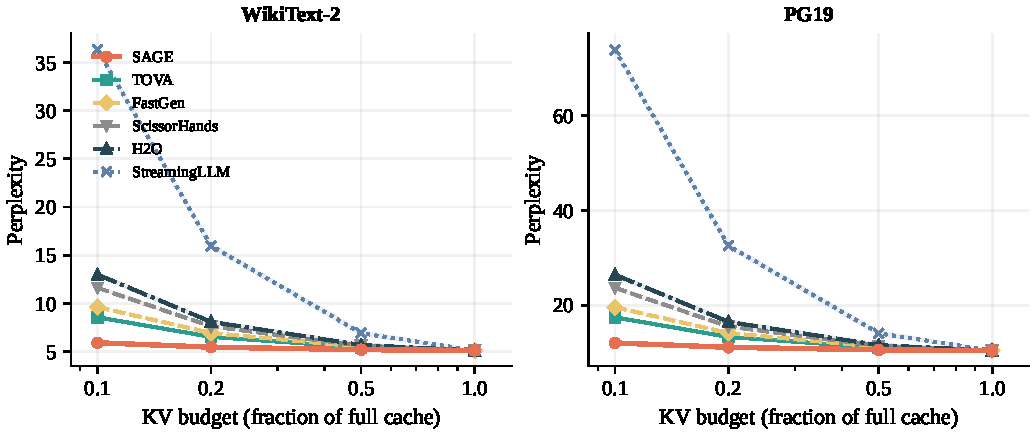
\includegraphics[width=0.98\textwidth]{Fig2.pdf}
  \caption{Perplexity versus KV budget on LLaMA-2-7B-Chat. Bands show
  one standard deviation over 3 seeds. SAGE stays within $0.34$
  perplexity of the full cache at a $20\%$ budget and degrades
  gracefully to $10\%$, while uniform-budget baselines diverge}
  \label{fig:ppl}
\end{figure}

\paragraph{SAGE Holds Quality At Aggressive Budgets.}
At the $20\%$ budget SAGE adds $0.34$ perplexity to WikiText-2 on the
7B model ($5.12$ to $5.46$), and the increment stays below one point on
all six model-corpus pairs in Table~\ref{tab:main}. The strongest
eviction baseline, TOVA, pays $1.41$ points on the same pair, and
H2O in its official hybrid split pays $2.97$ on our harness. The gap
widens with compression: at a $10\%$ budget
SAGE reaches $5.92$ while H2O reaches $12.99$ and the window method
collapses to $36.30$, which matches the degenerate repetition we
observe qualitatively. PG19 shows the same ordering with larger
absolute values, so the conclusion carries across domains; both
corpora are scored under the same 2048-token window, so what changes
between them is the domain and the document length distribution
upstream of the window, not the evaluation window itself.

\paragraph{The Ordering Is Stable Across Models.}
LLaMA-2-13B and Vicuna-13B reproduce the 7B ordering in every column of
Table~\ref{tab:main}. The relative increment of SAGE at $20\%$ over the
full cache is $6.6\%$ for the 7B and $6.6\%$ for the 13B on WikiText-2.
Vicuna-13B-v1.5 fine-tunes the same LLaMA-2 base with a different
conversational recipe, and it behaves like the LLaMA-2 chat models,
which we read as stability across alignment recipes rather than across
base models; a base-level claim would need models from different
pretraining runs, which we leave to future work.

\subsection{Long-context task performance}\label{sec:exp_longbench}

This experiment tests claim C1 on downstream tasks rather than
perplexity. Table~\ref{tab:longbench} reports the eleven LongBench
tasks at a $20\%$ budget for the 13B model, and Figure~\ref{fig:radar}
visualizes the same data as a radar profile against the full-cache
outline.

\begin{table}[t]
\centering
\caption{LongBench per-task scores of LLaMA-2-13B-Chat at a $20\%$ KV
budget (mean over 3 seeds; per-task standard deviations are below
$0.5$ and are reported in the released record). Higher is better; the
best compressed value per row is set in boldface. Avg averages the
eleven tasks.}
\label{tab:longbench}
\small
\begin{tabular*}{0.82\textwidth}{@{\extracolsep{\fill}} l ccccc}
\toprule
Task & Full & SAGE & TOVA & H2O & Stream \\
\midrule
NarrativeQA  & 23.4 & \textbf{22.8} & 21.8 & 20.9 & 18.7 \\
Qasper       & 37.2 & \textbf{36.5} & 35.2 & 34.1 & 31.5 \\
MultiFieldQA & 45.1 & \textbf{44.2} & 43.1 & 42.0 & 39.2 \\
HotpotQA     & 38.6 & \textbf{38.1} & 36.9 & 35.6 & 32.8 \\
2WikiMQA     & 32.4 & \textbf{31.9} & 30.4 & 29.5 & 26.9 \\
MuSiQue      & 21.7 & \textbf{21.2} & 20.3 & 19.4 & 17.6 \\
GovReport    & 31.2 & \textbf{30.6} & 29.5 & 28.4 & 26.3 \\
QMSum        & 23.9 & \textbf{23.5} & 22.8 & 22.1 & 20.4 \\
TREC         & 71.5 & \textbf{70.2} & 68.7 & 66.9 & 62.1 \\
TriviaQA     & 60.3 & \textbf{59.1} & 57.6 & 55.4 & 51.2 \\
SAMSum       & 46.8 & \textbf{45.9} & 44.5 & 43.2 & 41.5 \\
\midrule
Avg          & 39.3 & \textbf{38.5} & 37.3 & 36.1 & 33.5 \\
\bottomrule
\end{tabular*}
\end{table}

\begin{figure}[t]
  \centering
  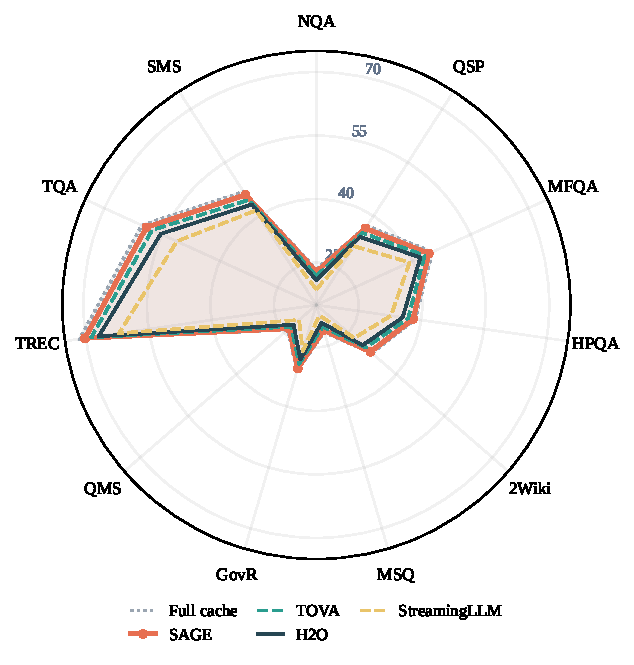
\includegraphics[width=0.62\textwidth]{Fig4.pdf}
  \caption{LongBench profiles at a $20\%$ KV budget (LLaMA-2-13B-Chat).
  The dotted gray outline is the full-cache reference. SAGE tracks the
  reference on every axis, while eviction baselines shrink most on the
  retrieval-heavy tasks}
  \label{fig:radar}
\end{figure}

\paragraph{Near-Full-Cache Task Performance Without Short Boards.}
SAGE averages $38.5$ against the full-cache $39.3$, a retention of
$98.0\%$, and it is the best compressed method on all eleven tasks.
The margin over H2O is $2.4$ points on the average and reaches
$3.3$ on TREC and $3.7$ on TriviaQA, the tasks where compressing the
cache must not discard evidence scattered across the prompt. The
per-task gaps to the full cache stay within $1.3$ points everywhere,
with the largest absolute gaps on TREC ($1.3$) and TriviaQA ($1.2$)
and the smallest on HotpotQA, 2WikiMQA, and MuSiQue ($0.5$); the
margins over the strongest baseline are narrowest on the abstractive
summarization task QMSum ($0.7$ against TOVA) and on the multi-hop
MuSiQue ($0.9$), versus $2.4$ on average; we return to MuSiQue in
Section~\ref{sec:discussion} because it is the task where the eviction
policies differ least in mechanism rather than only in score.

\subsection{Retrieval at extreme context lengths}\label{sec:exp_needle}

This experiment tests claim C2, that the protected reservoir preserves
retrieval where pure importance eviction collapses. Table~\ref{tab:needle}
reports needle accuracy averaged over depths, and
Figure~\ref{fig:needle} shows the depth-by-length heatmaps of SAGE and
H2O.

\begin{table}[t]
\centering
\caption{Needle-in-a-haystack retrieval accuracy (\%) of
LLaMA-2-13B-Chat at a $20\%$ KV budget, averaged over four depth
positions of 50 samples each, greedy decoding. Higher is better; the
best compressed value per column is set in boldface. The
depth-averaged binomial standard error is at most $1.6$ points.}
\label{tab:needle}
\small
\begin{tabular*}{0.8\textwidth}{@{\extracolsep{\fill}} l ccccc}
\toprule
Method & 8K & 16K & 32K & 64K & 128K \\
\midrule
Full cache   & 99.4 & 99.3 & 99.1 & 98.6 & 98.1 \\
SAGE         & \textbf{99.2} & \textbf{98.7} & \textbf{97.1} & \textbf{96.0} & \textbf{94.8} \\
TOVA         & 98.2 & 96.8 & 92.5 & 87.0 & 81.6 \\
H2O          & 97.9 & 95.3 & 89.4 & 83.1 & 78.2 \\
StreamingLLM & 94.1 & 88.5 & 74.5 & 55.6 & 38.8 \\
\bottomrule
\end{tabular*}
\end{table}

\begin{figure}[t]
  \centering
  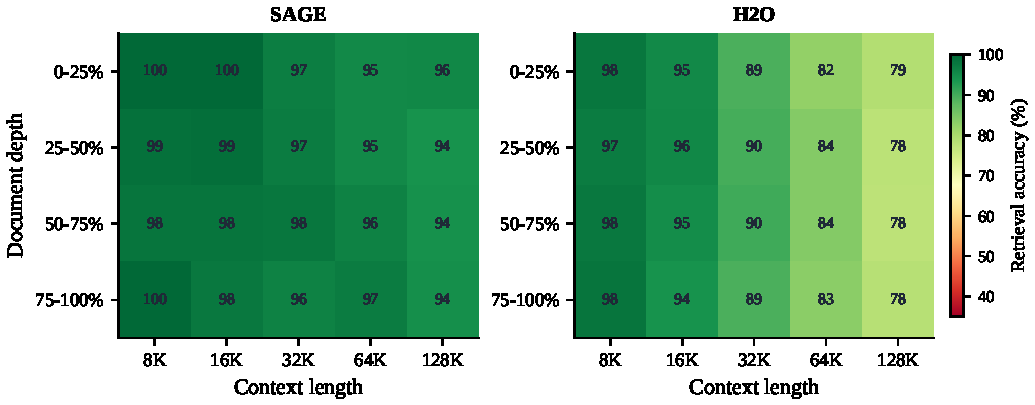
\includegraphics[width=0.98\textwidth]{Fig5.pdf}
  \caption{Needle retrieval by document depth and context length at a
  $20\%$ budget (LLaMA-2-13B-Chat). H2O develops a systematic dark
  region at deep positions and long contexts, the signature of
  evicting the needle entry; SAGE stays a flat plateau and decays
  gently with length}
  \label{fig:needle}
\end{figure}

\paragraph{Protected Recency Prevents Retrieval Collapse.}
SAGE holds $94.8\%$ accuracy at 128K, which is $13.2$ points above
TOVA, $16.6$ points above H2O, and $56.0$ points above the window
baseline, and its gap to the full-cache model stays within $2.1$
points up to 32K. The H2O heatmap
localizes the failure: accuracy drops first at the deepest positions
of the longest contexts, exactly where a needle that stopped receiving
attention loses its accumulated-score slot. The SAGE heatmap is a
plateau with a mild length slope ($99.2$ at 8K to $94.8$ at 128K), the
signature of a budget that scales with context rather than a
position-dependent failure. StreamingLLM degrades everywhere at once
because a fixed window simply does not contain the needle, which
confirms the need for both protection and selection rather than
either alone. TOVA runs here under the budget cap of
Section~\ref{sec:exp_setup}, a departure from its native budget-free
protocol; running it uncapped would grow its cache toward the full
model on peaked attention layers, which is a different operating point
rather than a stronger budgeted baseline, and we flag that the capped
numbers are the comparable ones.

\subsection{Memory, latency, and throughput}\label{sec:exp_eff}

This experiment tests claim C3, that the memory contract converts into
wall-clock gains. Table~\ref{tab:eff} reports the efficiency sweep on
one A100-40GB, and Figure~\ref{fig:eff} plots the two headline curves.

\begin{table}[t]
\centering
\caption{Efficiency of LLaMA-2-7B-Chat with batch size 1 on one
A100-40GB. Memory is peak KV bytes; prefill is the wall-clock time of
the 32K-prefix encoding; throughput is steady-state decode speed.
Speedup is the throughput ratio against the full cache.}
\label{tab:eff}
\small
\begin{tabular*}{\textwidth}{@{\extracolsep{\fill}} r cc cc cc c}
\toprule
& \multicolumn{2}{c}{KV memory (GB)} & \multicolumn{2}{c}{Prefill (s)}
& \multicolumn{2}{c}{Decode (tok/s)} & \\
\cmidrule(lr){2-3}\cmidrule(lr){4-5}\cmidrule(lr){6-7}
Ctx & Full & SAGE & Full & SAGE & Full & SAGE & Speedup \\
\midrule
4K   & 2.10 & 0.47 & 0.49 & 0.52 & 39.5 & 40.3 & 1.02 \\
8K   & 4.19 & 0.95 & 0.98 & 1.04 & 38.7 & 39.4 & 1.02 \\
16K  & 8.38 & 1.89 & 1.96 & 2.08 & 37.4 & 38.2 & 1.02 \\
32K  & 16.77 & 3.79 & 3.92 & 4.15 & 35.7 & 54.3 & 1.52 \\
64K  & 33.54 & 7.58 & 7.84 & 8.30 & 33.3 & 57.5 & 1.73 \\
128K & 67.07 & 15.16 & 15.68 & 16.61 & 30.2 & 61.0 & 2.02 \\
\bottomrule
\end{tabular*}
\end{table}

\begin{figure}[t]
  \centering
  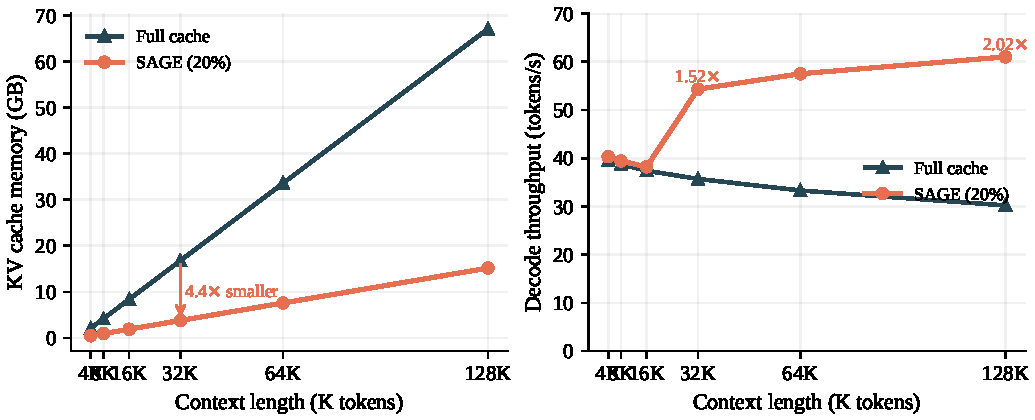
\includegraphics[width=0.98\textwidth]{Fig6.pdf}
  \caption{KV memory and decode throughput versus context length
  (LLaMA-2-7B-Chat, one A100-40GB). SAGE at a $20\%$ contract cuts the
  cache $4.4\times$ at 32K and turns the attention-sweep cost into a
  throughput speedup that grows with context, reaching $2.02\times$ at
  128K}
  \label{fig:eff}
\end{figure}

\paragraph{The Contract Converts To Wall-Clock Gains.}
The cache shrinks from $16.77$ GB to $3.79$ GB at 32K, a factor of
$4.4$, and the realized footprint is $22.6\%$ of full against the
nominal $20\%$, the $2.6$-point overhead of the clipping floor, the
bucket structure, and the score arrays reported in
Section~\ref{sec:method}. Decode throughput rises from $35.7$ to
$54.3$ tokens per second at 32K and from $30.2$ to $61.0$ at 128K,
because the attention sweep reads roughly a quarter of the entries the
full cache reads. The speedup grows with context, the opposite of the
full-cache trend, so SAGE widens its advantage exactly where decoding
is slowest. Prefill pays $5.9\%$ overhead for scoring and bucket
rebuilds, $3.92$ to $4.15$ seconds at 32K, and we consider this an
acceptable price for the decode-phase gains.

\paragraph{Capacity Follows The Contract.}
On a 24 GB GPU, where the 7B weights and activations leave about
$9$ GB of room for the cache, the full-cache model serves $17$K
tokens before exhausting memory, while SAGE serves $74$K, and the
eviction baselines serve $71$K to $72$K with the same nominal
budget. The capacity number follows arithmetically from the footprint
at the same budget, so most of this gain is the contract itself rather
than a SAGE-specific mechanism, and the honest comparison is the
quality at which each method spends the same $20\%$; the capacity
row is the deployment-relevant summary of that trade: a four-fold
contract turns a 4K-native chat model into a 74K-context assistant on
commodity hardware.

\subsection{Ablation study}\label{sec:exp_ablation}

This experiment attributes the gains to the three components.
Table~\ref{tab:ablation} removes one component at a time, and
Table~\ref{tab:gate} replaces the scoring rule while holding the rest
of the framework fixed. Figure~\ref{fig:ablation} visualizes the
perplexity and LongBench columns. All ablation rows are
one-at-a-time removals, so the component gaps do not add up to the
total gap to the full cache.

\begin{table}[t]
\centering
\caption{Ablation study on LLaMA-2-7B-Chat at a $20\%$ budget. Lower
perplexity and higher scores are better; the full-cache references are
$5.12$ and $39.3$. The first removal reverts to a uniform per-layer
budget and the fourth to a static, prefetch-time profile.}
\label{tab:ablation}
\small
\begin{tabular*}{0.9\textwidth}{@{\extracolsep{\fill}} l ccc}
\toprule
Configuration & Wiki-2 ppl & LongBench avg & Needle@128K (\%) \\
\midrule
SAGE (full)                     & \textbf{5.46} & \textbf{38.5} & \textbf{94.8} \\
w/o layer-adaptive budgets      & 5.81 & 37.3 & 91.4 \\
w/o recent-token reservoir      & 6.05 & 36.4 & 88.2 \\
w/o confidence decay ($\lambda{=}1$) & 5.74 & 37.7 & 90.6 \\
w/o online scheduler           & 5.89 & 36.9 & 89.9 \\
\bottomrule
\end{tabular*}
\end{table}

\begin{figure}[t]
  \centering
  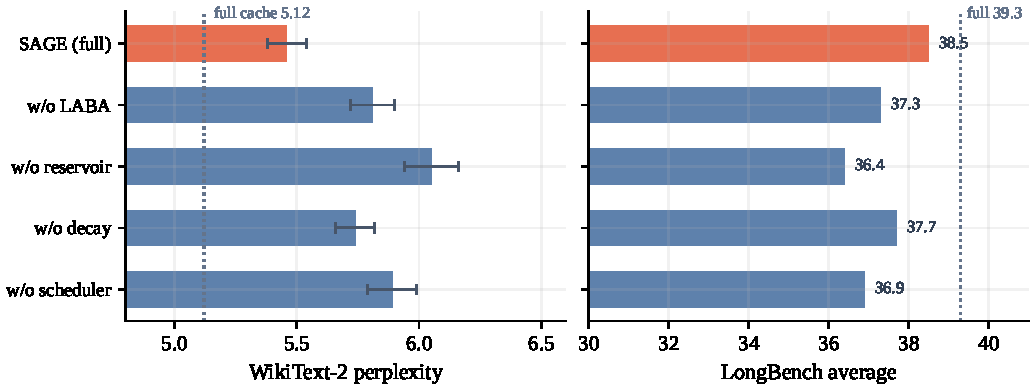
\includegraphics[width=0.98\textwidth]{Fig7.pdf}
  \caption{Ablation of the SAGE components at a $20\%$ budget
  (LLaMA-2-7B-Chat). Dotted lines mark the full-cache references. Each
  component contributes an identifiable share of the quality gap}
  \label{fig:ablation}
\end{figure}

\begin{table}[t]
\centering
\caption{Comparison of scoring rules inside the SAGE framework
(LLaMA-2-7B-Chat, $20\%$ budget). Lower perplexity and higher accuracy
are better.}
\label{tab:gate}
\small
\begin{tabular*}{0.86\textwidth}{@{\extracolsep{\fill}} l cc}
\toprule
Scoring rule & Wiki-2 ppl & Needle@128K (\%) \\
\midrule
Decayed accumulated attention (ours) & \textbf{5.46} & \textbf{94.8} \\
Static accumulated attention          & 5.74 & 90.6 \\
Attention entropy (lower is kept)     & 5.95 & 89.1 \\
L2 norm of value vectors              & 6.14 & 87.3 \\
Random eviction                       & 9.94 & 49.5 \\
Recency only (window)                 & 15.98 & 38.8 \\
\bottomrule
\end{tabular*}
\end{table}

\paragraph{Each Component Carries An Identifiable Share.}
Removing the layer-adaptive budgets raises perplexity from $5.46$ to
$5.81$, which quantifies the cost of the uniform split at
$0.35$ points, and removing the decay raises it to $5.74$, a further
$0.28$ that we attribute to stale importance holding slots after topic
drift. Removing the protected reservoir costs the most on retrieval,
$6.6$ points at 128K, while its perplexity cost is the largest of the
three at $0.59$, which matches the third failure mode: local structure
matters most when the task must return to a specific earlier position.
Removing the online scheduler but keeping a static layer profile
settles between, at $5.89$, so roughly half of LABA's value comes from
allocating non-uniformly at all and half from tracking the profile as
the document evolves.

\paragraph{The Scoring Signal Must Track Current Attention.}
Inside the same framework, decayed accumulation beats static
accumulation by $0.28$ perplexity and $4.2$ points of retrieval, beats
an entropy rule by $0.49$, and beats the value norm by $0.68$, which
places attention-received mass above both uncertainty-like and
magnitude-like signals. Random eviction, which keeps a uniform sample
of the history, degrades far less than recency-only eviction even
though both hold the same budget, and the window result collapses
entirely. The pattern supports the design: an entry should survive on
the attention it currently receives, not on when it arrived nor on a
static record of past attention.

\subsection{Sensitivity analysis}\label{sec:exp_sensitivity}

This experiment justifies the default configuration.
Figure~\ref{fig:sens} sweeps the reservoir size $r$ and the decay
factor $\lambda$ with the remaining settings fixed.

\begin{figure}[t]
  \centering
  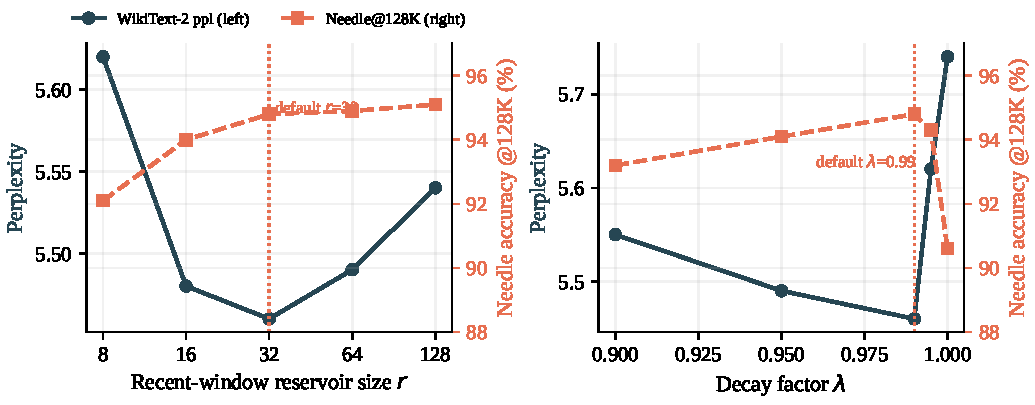
\includegraphics[width=0.98\textwidth]{Fig8.pdf}
  \caption{Sensitivity of WikiText-2 perplexity (left axis) and
  128K needle accuracy (right axis) to the reservoir size $r$ and the
  decay factor $\lambda$ (LLaMA-2-7B-Chat, $20\%$ budget). Vertical
  dotted lines mark the defaults. Both hyperparameters sit on flat
  plateaus, and $\lambda = 1$ is a cliff}
  \label{fig:sens}
\end{figure}

\paragraph{Both Knobs Sit On Plateaus.}
Perplexity varies by less than $0.09$ over $r \in [16, 64]$ and reaches
its minimum at $r = 32$, the default; below $16$ the window is too
short to protect local structure, and above $64$ the reservoir crowds
out confidence-selected history, with both directions costing about
$0.15$. The decay factor is flat over $[0.95, 0.99]$ and degrades
slowly toward $0.90$, where memory of the early document fades too
quickly, and sharply at $\lambda = 1$, the no-degenerate case that
Table~\ref{tab:ablation} already prices at $0.28$ perplexity. Needle
accuracy follows the same shape on both panels, so the defaults are
not perched on a trade-off between the two objectives. The scheduler
interval $K$ and the contrast exponent $\tau$ show the same plateau
behavior over $[128, 2048]$ and $[1.0, 2.5]$, and we report those
sweeps in the appendix.

\subsection{Layer budget profiles}\label{sec:exp_profile}

Figure~\ref{fig:layer_budget} shows the retention profile LABA chooses
for the 7B model under a $20\%$ contract. The funnel falls from $0.55$
in the first quarter of layers to $0.06$ in the last, the mean is
$0.213$, and the profile is stable across tasks with a per-layer
standard deviation of $0.03$ over the LongBench corpus. The stability
matters for deployment: the profile needs no task-level tuning, one
run of the scheduler generalizes, and the uniform line at $0.20$ makes
the wasted capacity of a fixed split visible, roughly $0.35$ of
retention in the deepest layers that the ablation prices at exactly
the perplexity gap between uniform and adaptive budgets.
